\documentclass[a4paper, fleqn]{report}

\usepackage[T2A]{fontenc}
\usepackage[utf8]{inputenc}
\usepackage[russian]{babel}

\usepackage{amsmath}
\usepackage{geometry}
\usepackage{graphicx}
\usepackage{hyperref}
\usepackage{enumitem}
\usepackage{listings}
\usepackage{titlesec}
\usepackage{tocbibind}
\usepackage{xcolor}
\usepackage{subcaption}

\geometry{top=2cm, bottom=2cm, left=2.5cm, right=2.5cm}

\hypersetup{
    colorlinks=true,
    linkcolor=blue,
    urlcolor=blue
}

\titleformat{\chapter}[block]
{\normalfont\huge\bfseries}{}{0em}{}

\lstset{
    basicstyle=\ttfamily\footnotesize,
    keywordstyle=\bfseries\color{blue},
    commentstyle=\itshape\color{gray},
    stringstyle=\color{red},
    numbers=left,
    numberstyle=\small,
    stepnumber=1,
    breaklines=true,
    frame=single,
    tabsize=4,
    captionpos=b,
}

\title{
\textbf{Московский Государственный Университет имени М.В.\ Ломоносова}\\
\textbf{Факультет вычислительной математики и кибернетики}\\
\textbf{Введение в численные методы}\\
Отчёт по практическому заданию
}

\author{
Студент: Борисов Тимофей, 207 группа
}
\date{\number\year}

\begin{document}

\maketitle

\tableofcontents

\chapter{Содержание отчёта о выполнении задания по численным методам}

\section*{Задание и краткое описание работы}
\addcontentsline{toc}{section}{Задание и краткое описание работы}

В рамках задания №2 необходимо:
\begin{enumerate}
    \item Построить полином Лагранжа для двух функций: \( f_1 \) и \( f_2 \) на отрезке \([0, 2]\). Количество узлов для интерполяции берётся равным 3, 5, 9 и 17.
    \item Для функции \( f_2 \) дополнительно применить еще один численный метод, который нужно было выбрать самостоятельно (в моем случае - метод интерполяции сплайнами).
    \item Исследовать интерполяции на сходимость.
    \item Найти максимальное отклонение интерполяции на равномерной сетке, состоящей из 1001 узла на отрезке \([0, 2]\).
    \item Построить графики функций и их интерполянтов.
\end{enumerate}

\newpage

\chapter{Описание используемых численных методов}

\section{Построение интерполяционного полинома Лагранжа}

\textbf{Идея метода.} Для заданных узлов \( x_0, x_1, \ldots, x_n \) и значений функции \( f(x_i) \) строится полиномиальная функция \( P_n(x) \), которая в точности совпадает с \( f(x) \) во всех этих узлах:
\[
P_n(x_i) = f(x_i), \quad i = 0,1,\ldots,n.
\]
Полином Лагранжа имеет вид:
\[
P_n(x) = \sum_{i=0}^{n} f(x_i) \, L_i(x),
\]
где \(\displaystyle L_i(x)\) --- \textit{базисные полиномы, "ориентированные" в узлах заданной сетки}:
\[
L_i(x) = \prod_{\substack{0 \,\le\, j \,\le\, n \\ j \,\neq\, i}} \frac{x - x_j}{x_i - x_j}.
\]
Каждый \( L_i(x) \) обращается в 0 при \( x = x_j \) (для \( j \neq i \)) и равен 1 при \( x = x_i \).

\vspace{10pt}

\textbf{Преимущества}:
\begin{itemize}
    \item Простота реализации: достаточно записать явную формулу и циклы.
    \item Точность высока, если узлы выбираются «удачно» (например, узлы Чебышева) и их не слишком много.
\end{itemize}

\textbf{Недостатки}:
\begin{itemize}
    \item Если количество узлов слишком большое, то и нарушается точность вычислений. Возникает феномен Рунге для полиномов больших степеней.
    \item Если нужно добавить новый узел, то приходится перестраивать полином заново.
    \item При больших осцилляциях (колебаниях) функции (как на 2 наборе данных), возникают также слишком большие отклонения в вычислениях (особенно ближе к границам интервала). 
\end{itemize}



Поэтому, для второго набора данных, я использовал метод кубических сплайнов.

\section{Интерполяция кубическими сплайнами}


При кубической сплайн-интерполяции весь отрезок \([a, b]\) разбивается на подотрезки \linebreak \([x_0, x_1], [x_1, x_2], \ldots, [x_{n-1}, x_n]\). На каждом подотрезке интерполяционная функция представляется полиномом третьей степени. Такой полином \( S_i(x) \) удовлетворяет условиям:
\[
S_i(x_i) = f(x_i), \quad i = 0, \dots, n,
\]
а также должны быть непрерывны первые и вторые производные на стыках, что дает следующие условия:
\[
S_i(x_i) = S_{i-1}(x_i), \quad S'_i(x_i) = S'_{i-1}(x_i), \quad S''_i(x_i) = S''_{i-1}(x_i) \quad i = 1, \dots, n.
\]
Также накладываются \textit{натуральные} граничные условия \( S''(x_0) = 0 \) и \( S''(x_n) = 0 \).

\vspace{10pt}

\noindent Кубический сплайн на сегменте \([x_{i-1}, x_i]\) удобно записать в таком виде:
\[
S_i(x) = a_i + b_i(x - x_i) + \frac{c_i}{2}(x - x_i)^2 + \frac{d_i}{6}(x - x_i)^3, \quad x \in [x_{i-1}, x_i], \; i = 1, \ldots, n. \tag ={*}
\]
Из системы уравнений 
\[
c_{i-1} + 4c_i + c_{i+1} = 6 \frac{f_{i-1} - 2f_i +f_{i+1}}{h^2}, \quad i = 1, \dots, n-1. \tag ={**}
\]
и имея граничные условия
\[
c_0 = 0, \quad c_n = 0
\]
мы можем найти все коэффициенты \(c_i, \quad i = 1, \dots, n\).

\vspace{10pt}

\noindent Коэффициенты \(d_i, \quad i = 1, \dots, n-1\) можно найти из соотношений
\[
d_i = \frac{c_i - c_{i-1}}{h}, \quad i = 1, \dots, n
\]
и коэффициенты \(b_i, \quad i = 1, \dots, n-1\) \quad - из соотношений
\[
b_i = \frac{1}{2}hc_i - \frac{1}{6}h^2d_i + \frac{f_i - f_{i-1}}{h}, \quad i = 1, \dots, n.
\]
При этом:
\[
a_i = f_i, \quad i = 1, \dots, n.
\]
Систему (**) можно решить с помощью метода прогонки, предполагая, что:
\begin{equation}
    \ c_i = \alpha_{i+1}c_{i+1} + \beta_{i+1}, \quad i = 0, \dots, n - 1;
\end{equation}
\begin{equation}
    \alpha_{i+1} =\frac{-B_i}{A_i\alpha_i + C_i}, \quad \beta_{i+1} =\frac{F_i - A_i\beta_i}{A_i\alpha_i + C_i}, \quad i = 1, \dots, n-1.\
\end{equation}

\vspace{10pt}

\noindent Таким образом, мы можем найти значение сплайна в любой точке х, зная все нужные коэффициенты \(a_i, b_i, c_i, d_i\).

\vspace{10pt}

\textbf{Преимущества метода интерполяции сплайнами}:
\begin{itemize}
    \item Нет эффекта Рунге, поскольку используется кусочно-полиномиальная интерполяция невысокого (3) порядка.
    \item При добавлении новых узлов пересчитываются только «локальные» коэффициенты (не нужно перестраивать глобальный полином).
\end{itemize}

\textbf{Недостатки}:
\begin{itemize}
    \item Более сложная реализация: необходимо решать систему линейных уравнений для получения коэффициентов \( c_i \).
    \item Из-за разных вариантов граничных условий их нужно подбирать корректно в зависимости от задачи.
\end{itemize}

\chapter{Сходимость интерполяционного процесса}

Чтобы оценить качество интерполяции, часто рассматривают:
\[
\max_{x \in [a, b]} \bigl|P_n(x) - f(x)\bigr|,
\]
где \(P_n\) --- построенный интерполянт. Если увеличить число узлов \(n\) (и при этом разбивать интервал более «грамотно»), то норма ошибки должна убывать. Для сплайнов аналогично:
\[
\max_{x \in [a, b]} |S(x) - f(x)|.
\]

На практике удобнее смотреть на несколько «промежуточных» точек (не входящих в узлы), измерять отклонение там, а затем находить максимум. В нашем случае, оба интерполяционных процесса сходятся. Но сходимость интерполяции сплайнами особенно быстрая, соответственно, этот метод дает более точное приближение.

\chapter{Программная реализация и результаты}

\section*{Описание кода}

В моей программе (написана на языке C) реализованы следующие блоки:
\begin{itemize}
    \item \textbf{Функции} \(f_1\) и \(f_2\), для которых необходимо построить графики интерполянтов, а также графики и самих функций. Отрезок задан: \([0, 2]\).
    \item \textbf{Построение полинома Лагранжа.} Функция \(\texttt{Lagrange\_polynomial}(\dots)\) вычисляет значение полинома Лагранжа в какой-либо точке x на отрезке \([0, 2]\). Функция вызывается в цикле столько раз, сколько задано точек узлов сетки (по умолчанию графики строятся для 101 точки, но пользователь может ввести и другое значение).
    \item \textbf{Вычисление коэффициентов для кубических сплайнов:} функция \(\texttt{cubic\_spline}(\dots)\) вычисляет коэффициенты для сплайнов (для этого вызывает внутри себя другие функции), затем вычисляет значение сплайна в точке х. Коэффициенты находятся в процессе решения системы уравнений, матрица которой имеет трехдиагональную форму. Сначала вычисляются \(c_i\), затем идет последующее восстановление \((a_i, b_i, c_i, d_i)\) для каждого сегмента сплайна.
    \item \textbf{Создание файлов:} после всех вычислений функций, а также их интерполянтов, создается текстовый файл (формат \texttt{.dat}) в который записывается множество точек для каждой функции. После этого происходит визуализация получившихся данных в gnuplot (в папке graphs сохранены графики функций).
    \item \textbf{Печать максимальных отклонений интерполянтов:} в последнюю очередь, после создания файлов, печатаются значения максимальных отклонений интерполянтов от самих функций. Программа сравнивает их значения на сетке из 1001 узлов и сохраняет результат, после чего печатает. Сначала идет печать четырех значений для первой функции, затем четырех значений для второй.
\end{itemize}
\section*{Результаты вычислений}
Как уже было сказано ранее, программа создает несколько текстовых файлов с наборами данных для каждоый функции и её интерполянта (для первой функции - полиномы Лагранжа, для второй - данные, полученые для сплайнов). Результаты работы программы находятся в репозитории. Названия файлов имеюи следующий вид: \(\texttt{fi\_type\_n}\), где \(i\) - номер функции, \(\texttt{type}\) - тип интерполянта (\(\texttt{poly}\) - полином Лагранжа, \(\texttt{spln}\) - кубический сплайн), \(\texttt{n}\) - количество узлов сетки, для которой строится интерполяция (сетка равномерная). Файлы \(\texttt{f1.dat}\) и \(\texttt{f2.dat}\) - файлы, имеющие наборы данных для исходных функций, для которых решается задача интерполяции. 
Для первой функции применение полинома Лагранжа дает не очень корректный результат: возле краев отрезка приближение было неточным, были большие колебания

\clearpage

\begin{table}[h!]
\centering
\begin{subtable}{0.45\textwidth}
\centering
\begin{tabular}{|c|c|}
\hline
X & Y \\ \hline
0.000000 & 0.000000 \\ \hline
0.100000 & -8.168750 \\ \hline
0.200000 & -14.500000 \\ \hline
0.300000 & -18.993750 \\ \hline
0.400000 & -21.650000 \\ \hline
0.500000 & -22.468750 \\ \hline
0.600000 & -21.450000 \\ \hline
0.700000 & -18.593750 \\ \hline
0.800000 & -13.900000 \\ \hline
0.900000 & -7.368750 \\ \hline 
1.000000 & 1.000000 \\ \hline
1.100000 & 11.206250 \\ \hline
1.200000 & 23.250000 \\ \hline
1.300000 & 37.131250 \\ \hline
1.400000 & 52.850000 \\ \hline
1.500000 & 70.406250 \\ \hline
1.600000 & 89.800000 \\ \hline
1.700000 & 111.031250 \\ \hline
1.800000 & 134.100000 \\ \hline
1.900000 & 159.006250 \\ \hline
2.000000 & 185.750000 \\ \hline
\end{tabular}
\caption{\texttt{f1\_poly\_3.dat}}
\label{tab:table1}
\end{subtable}%
\hspace{0.01\textwidth} % Пробел между таблицами
\begin{subtable}{0.45\textwidth}
\centering
\begin{tabular}{|c|c|}
\hline
X & Y \\ \hline
0.000000 & 0.000000 \\ \hline
0.100000 & 0.178829 \\ \hline
0.200000 & 0.307520 \\ \hline
0.300000 & 0.345386 \\ \hline 
0.400000 & 0.270640 \\ \hline
0.500000 & 0.089844 \\ \hline
0.600000 & -0.152640 \\ \hline
0.700000 & -0.365199 \\ \hline
0.800000 & -0.399520 \\ \hline
0.900000 & -0.041141 \\ \hline
1.000000 & 1.000000 \\ \hline
1.100000 & 3.099016 \\ \hline
1.200000 & 6.725520 \\ \hline
1.300000 & 12.453074 \\ \hline
1.400000 & 20.968640 \\ \hline
1.500000 & 33.082031 \\ \hline
1.600000 & 49.735360 \\ \hline
1.700000 & 72.012489 \\ \hline
1.800000 & 101.148480 \\ \hline
1.900000 & 138.539046 \\ \hline
2.000000 & 185.750000 \\ \hline
\end{tabular}
\caption{\texttt{f1\_poly\_17.dat}}
\label{tab:table2}
\end{subtable}
\vspace{10pt}
\caption{Примеры данных для двух файлов в виде таблицы (полином Лагранжа)}
\label{tab:both_tables}
\end{table}

\vspace{10pt}

\noindent \textbf{Пример вывода программы (n = 101):}

\vspace{10pt}

\begin{verbatim}
Enter number of dots for graphs: 101
---
All data files were successfully created
---
Max deviation for f1 and Lagrange polynomial (n = 3): 40.204123
Max deviation for f1 and Lagrange polynomial (n = 5): 0.893672
Max deviation for f1 and Lagrange polynomial (n = 9): 0.000000
Max deviation for f1 and Lagrange polynomial (n = 17): 0.000000
---
Max deviation for f2 and cubic spline (n = 3): 29.435939
Max deviation for f2 and cubic spline (n = 5): 9.883389
Max deviation for f2 and cubic spline (n = 9): 7.335909
Max deviation for f2 and cubic spline (n = 17): 3.740584
---
\end{verbatim}


\begin{figure*}[h]
    \centering
    \begin{minipage}{0.8\textwidth}
        \centering
        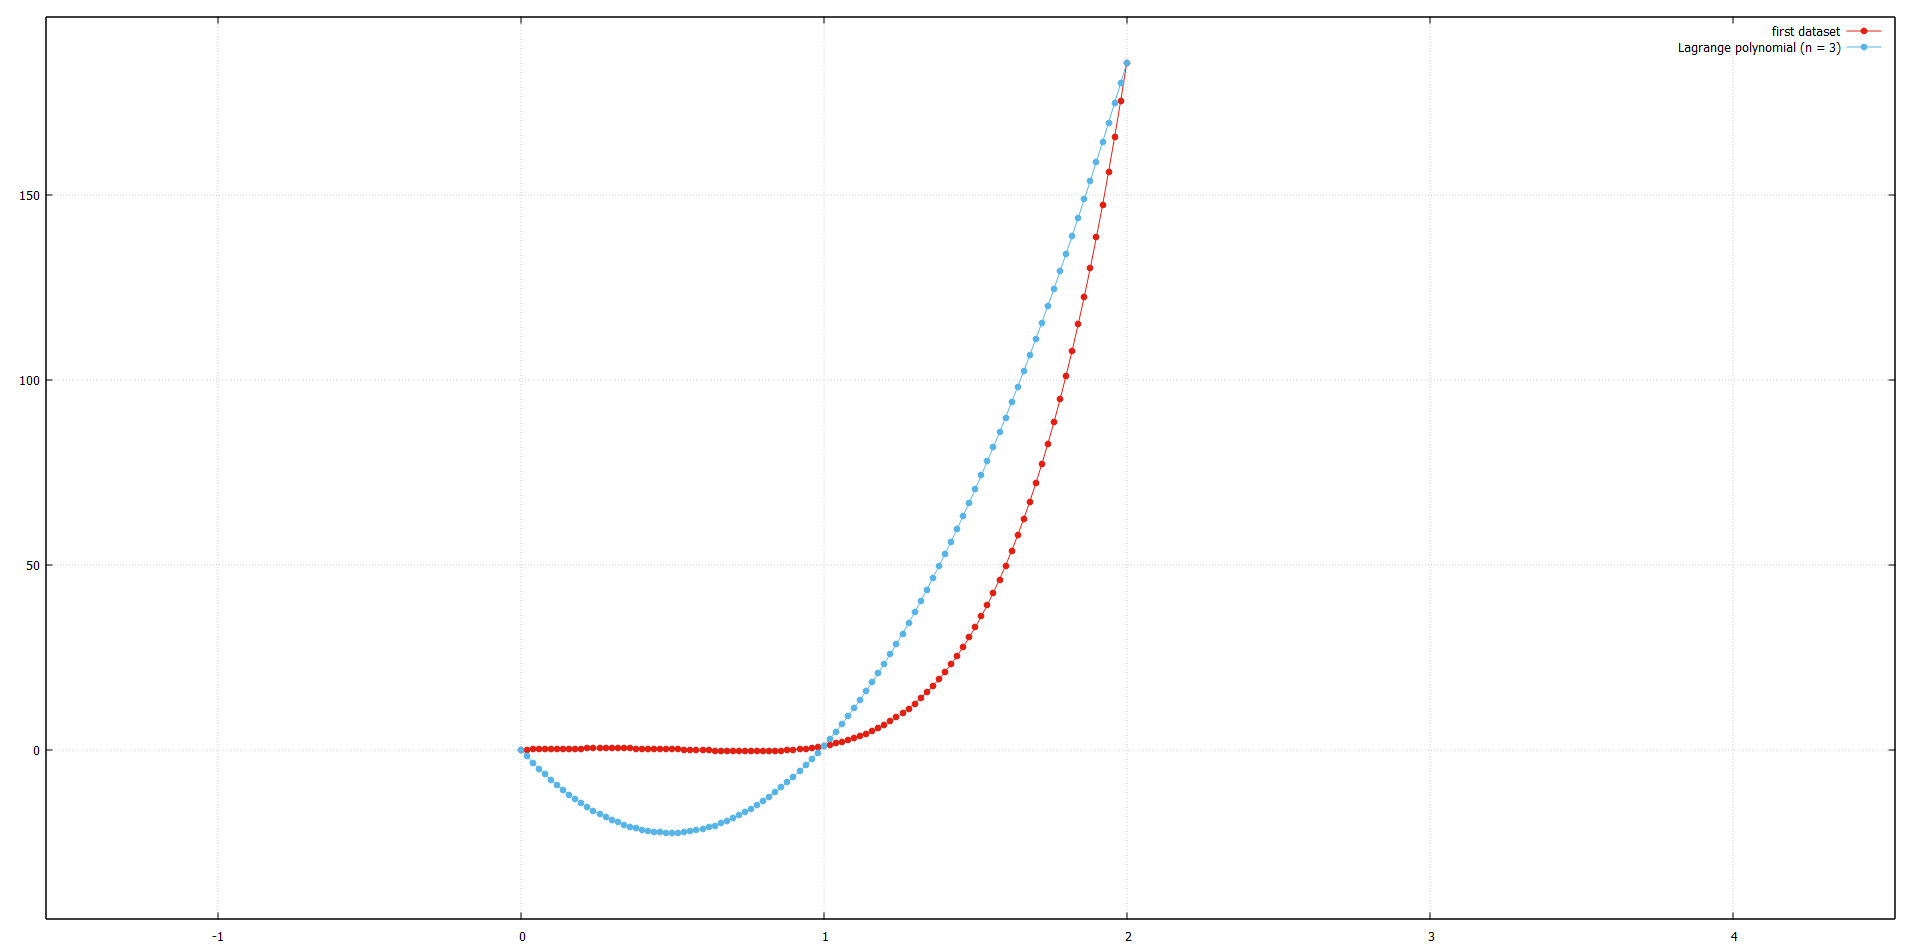
\includegraphics[width=\textwidth]{graph/f1_3.png}
        \caption{Lagrange polynomial (n = 3)}
    \end{minipage}%
\end{figure*}
\begin{figure*}[h]
    \centering
    \begin{minipage}{0.8\textwidth}
        \centering
        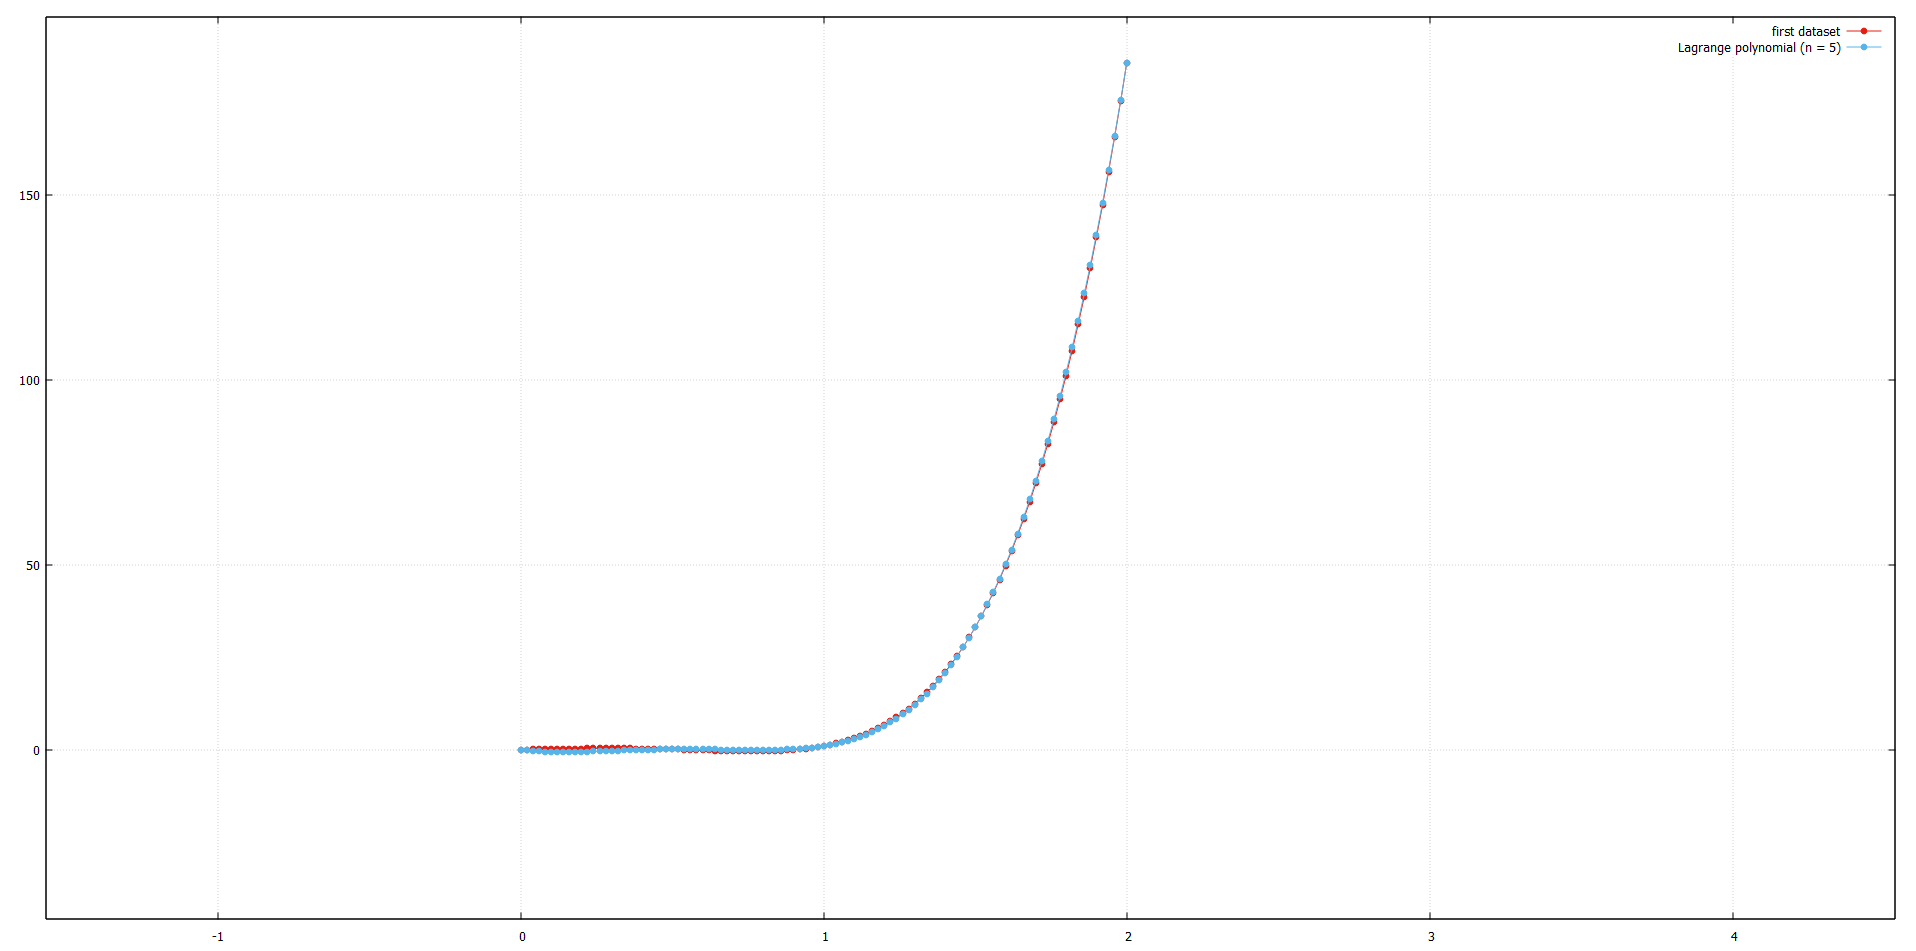
\includegraphics[width=\textwidth]{graph/f1_5.png}
        \caption{Lagrange polynomial (n = 5)}
    \end{minipage}%
\end{figure*}
\begin{figure*}[h]
    \centering
    \begin{minipage}{0.8\textwidth}
        \centering
        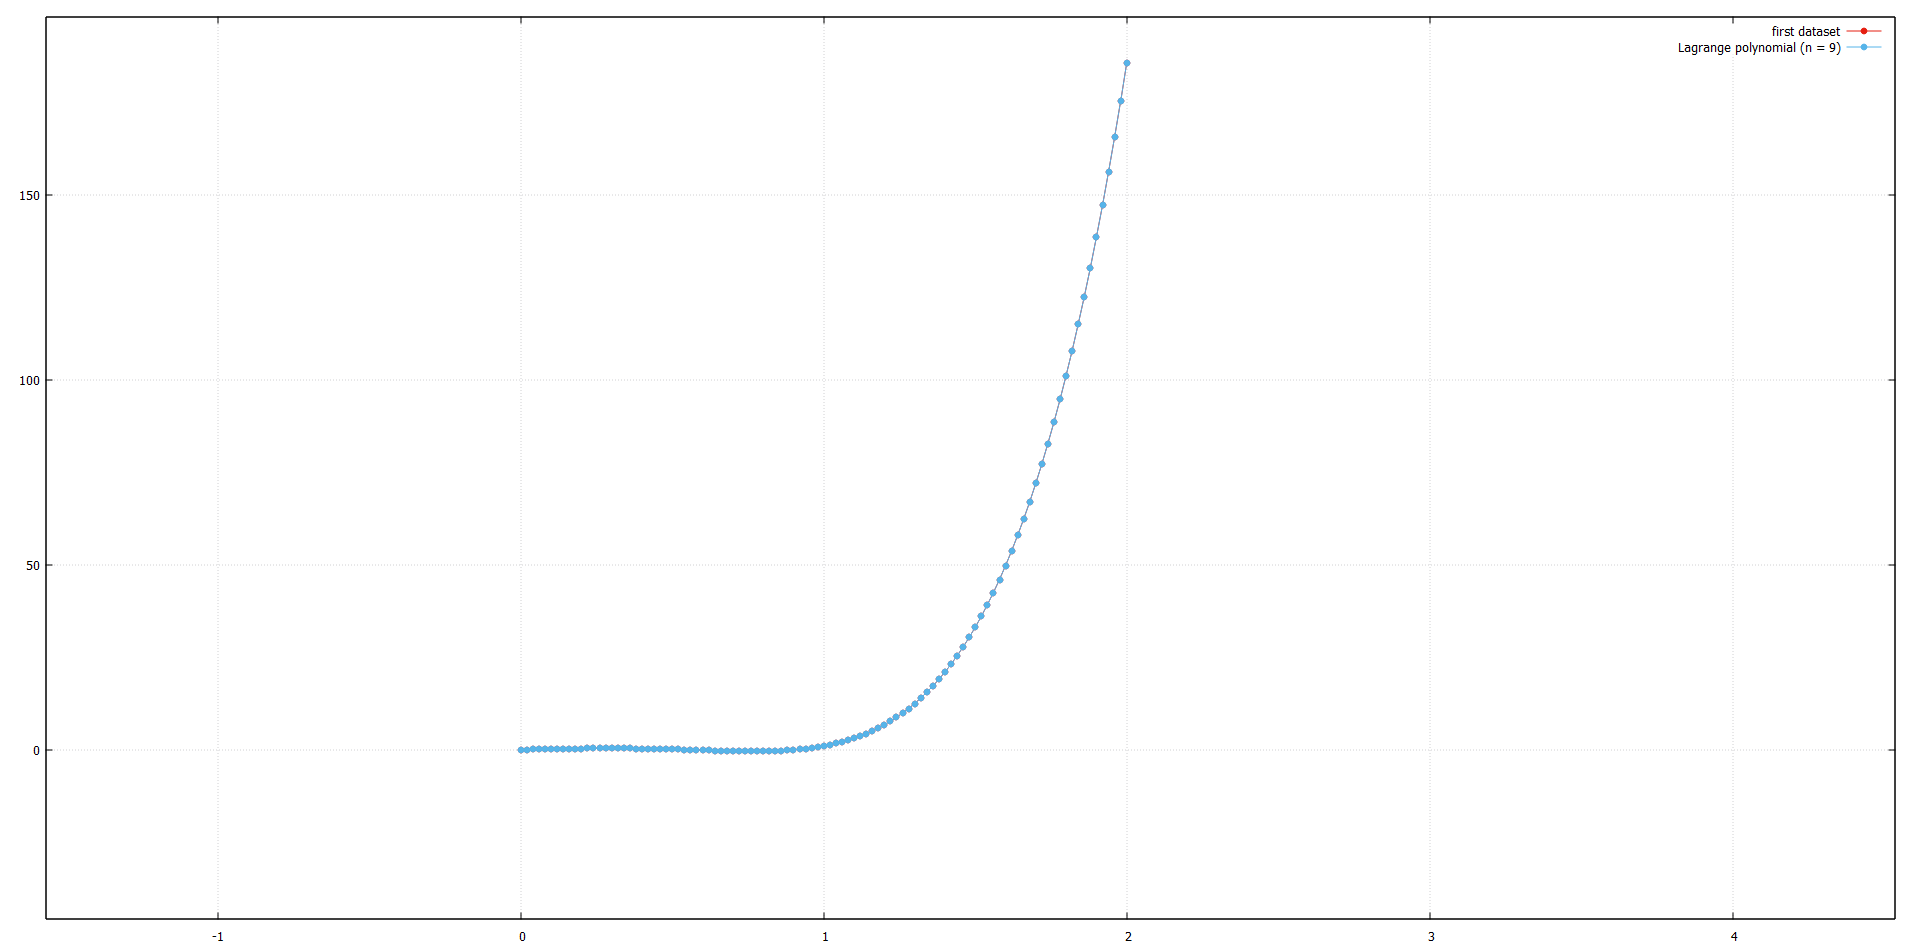
\includegraphics[width=\textwidth]{graph/f1_9.png}
        \caption{Lagrange polynomial (n = 9)}
    \end{minipage}%
\end{figure*}
\begin{figure*}[h]
    \centering
    \begin{minipage}{0.8\textwidth}
        \centering
        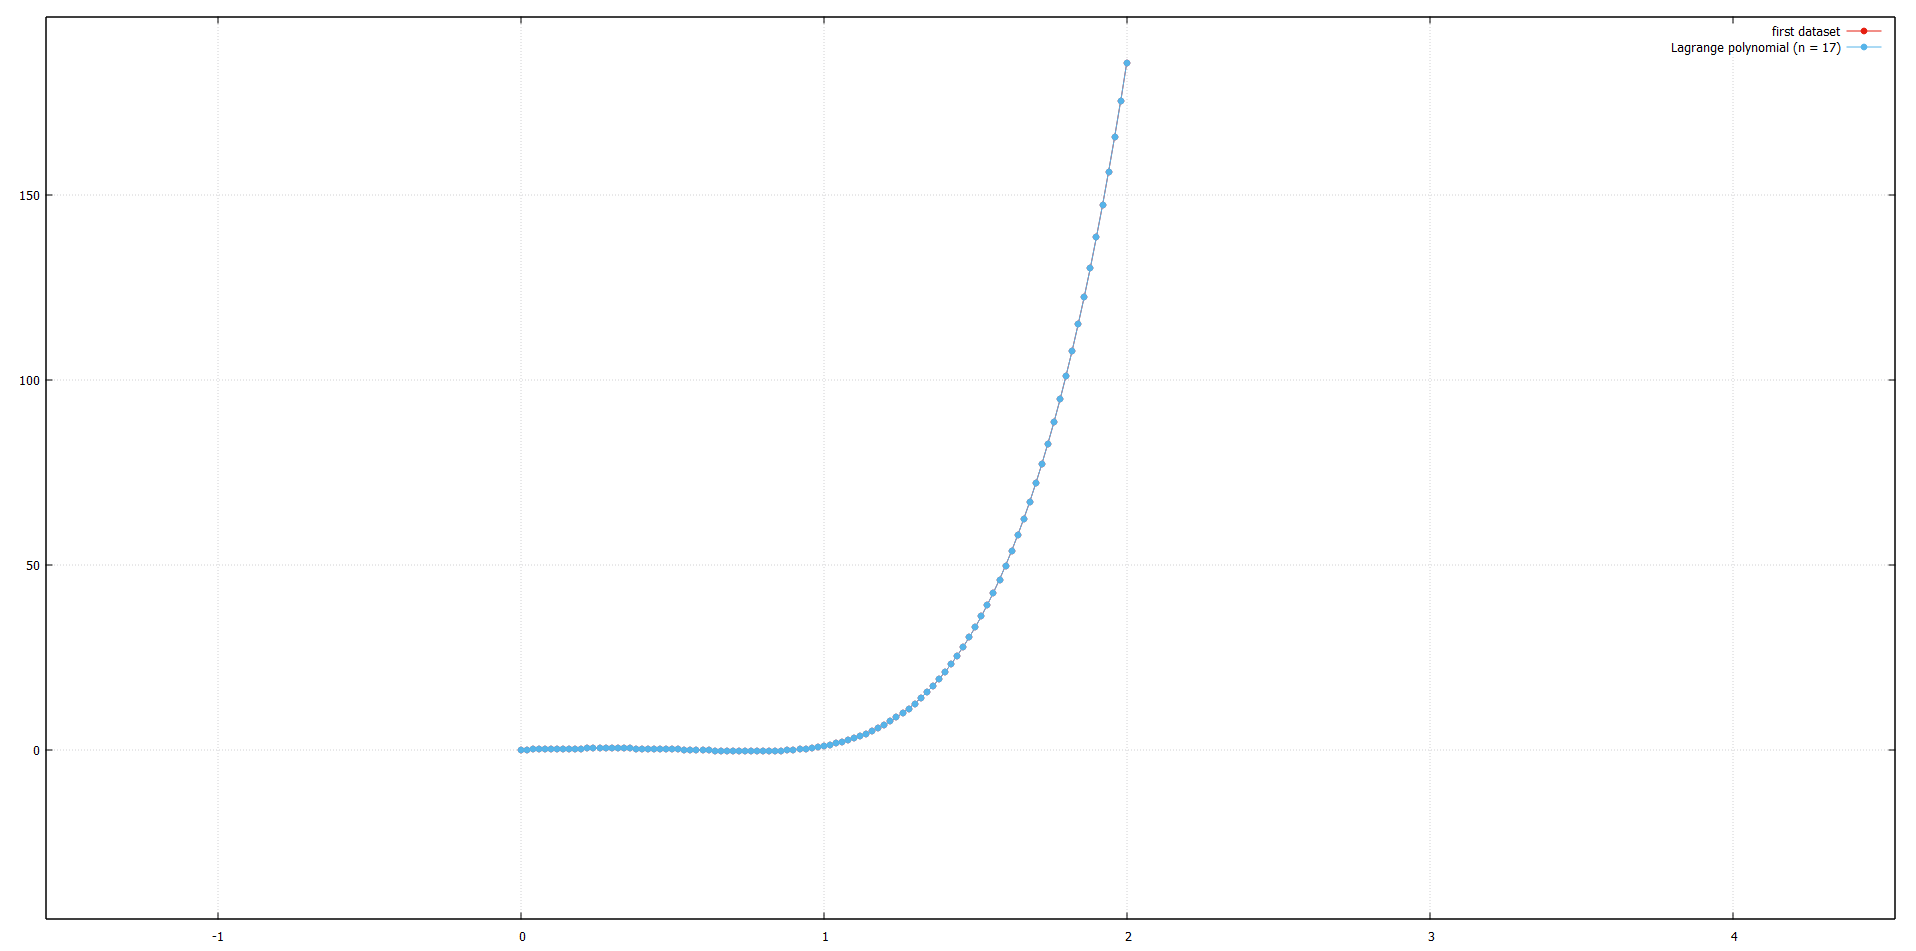
\includegraphics[width=\textwidth]{graph/f1_17.png}
        \caption{Lagrange polynomial (n = 17)}
    \end{minipage}%
\end{figure*}
\begin{figure*}[h]
    \centering
    \begin{minipage}{0.8\textwidth}
        \centering
        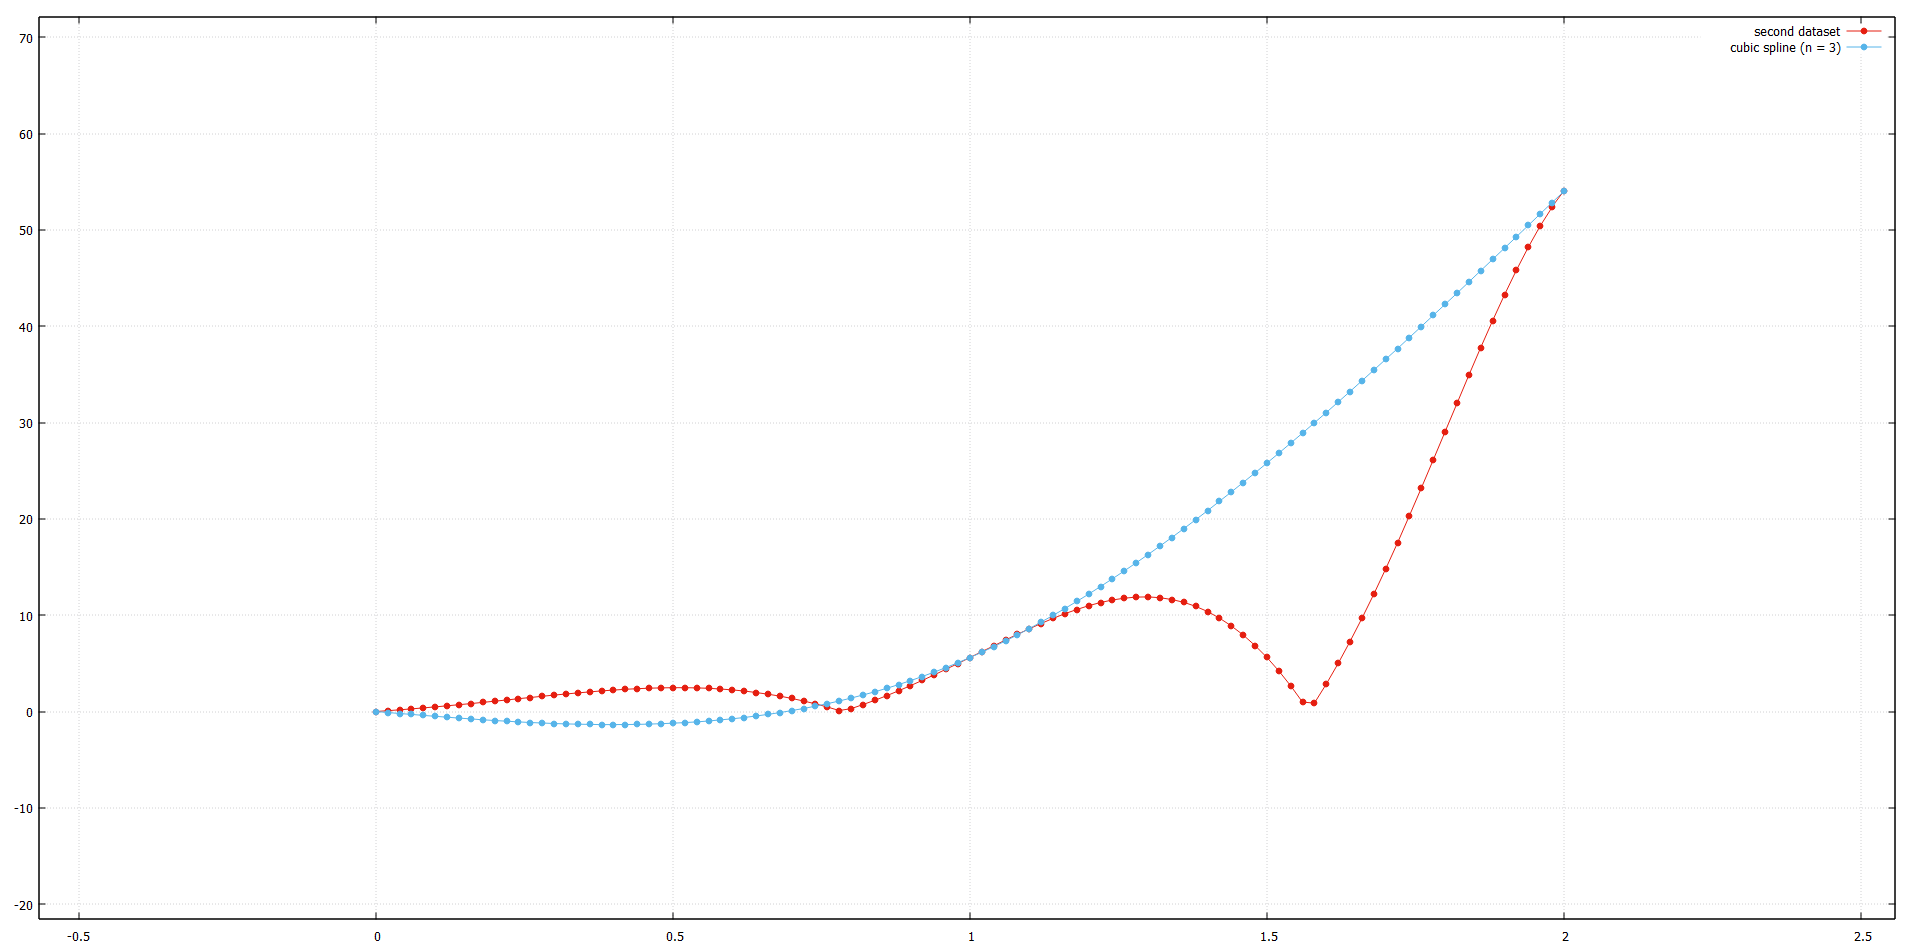
\includegraphics[width=\textwidth]{graph/f2_3.png}
        \caption{Cubic spline (n = 3)}
    \end{minipage}%
\end{figure*}
\begin{figure*}[h]
    \centering
    \begin{minipage}{0.8\textwidth}
        \centering
        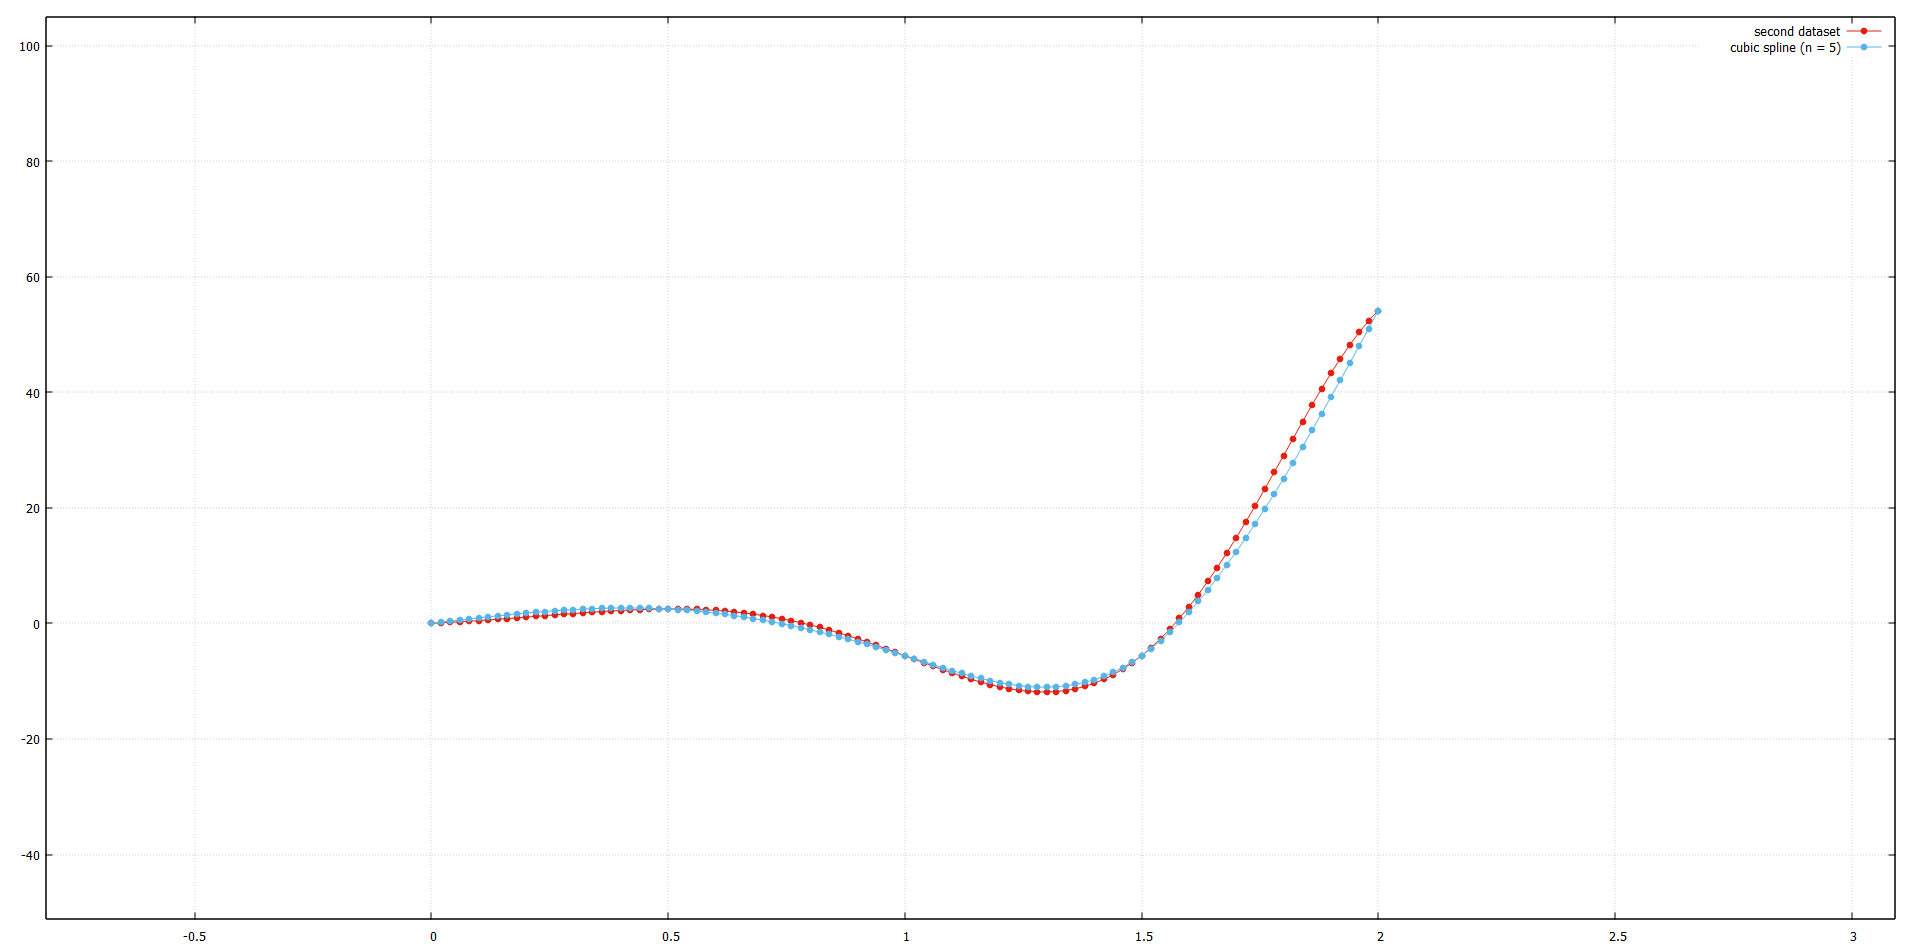
\includegraphics[width=\textwidth]{graph/f2_5.png}
        \caption{Cubic spline (n = 5)}
    \end{minipage}%
\end{figure*}
\clearpage
\begin{figure*}[h]
    \centering
    \begin{minipage}{0.8\textwidth}
        \centering
        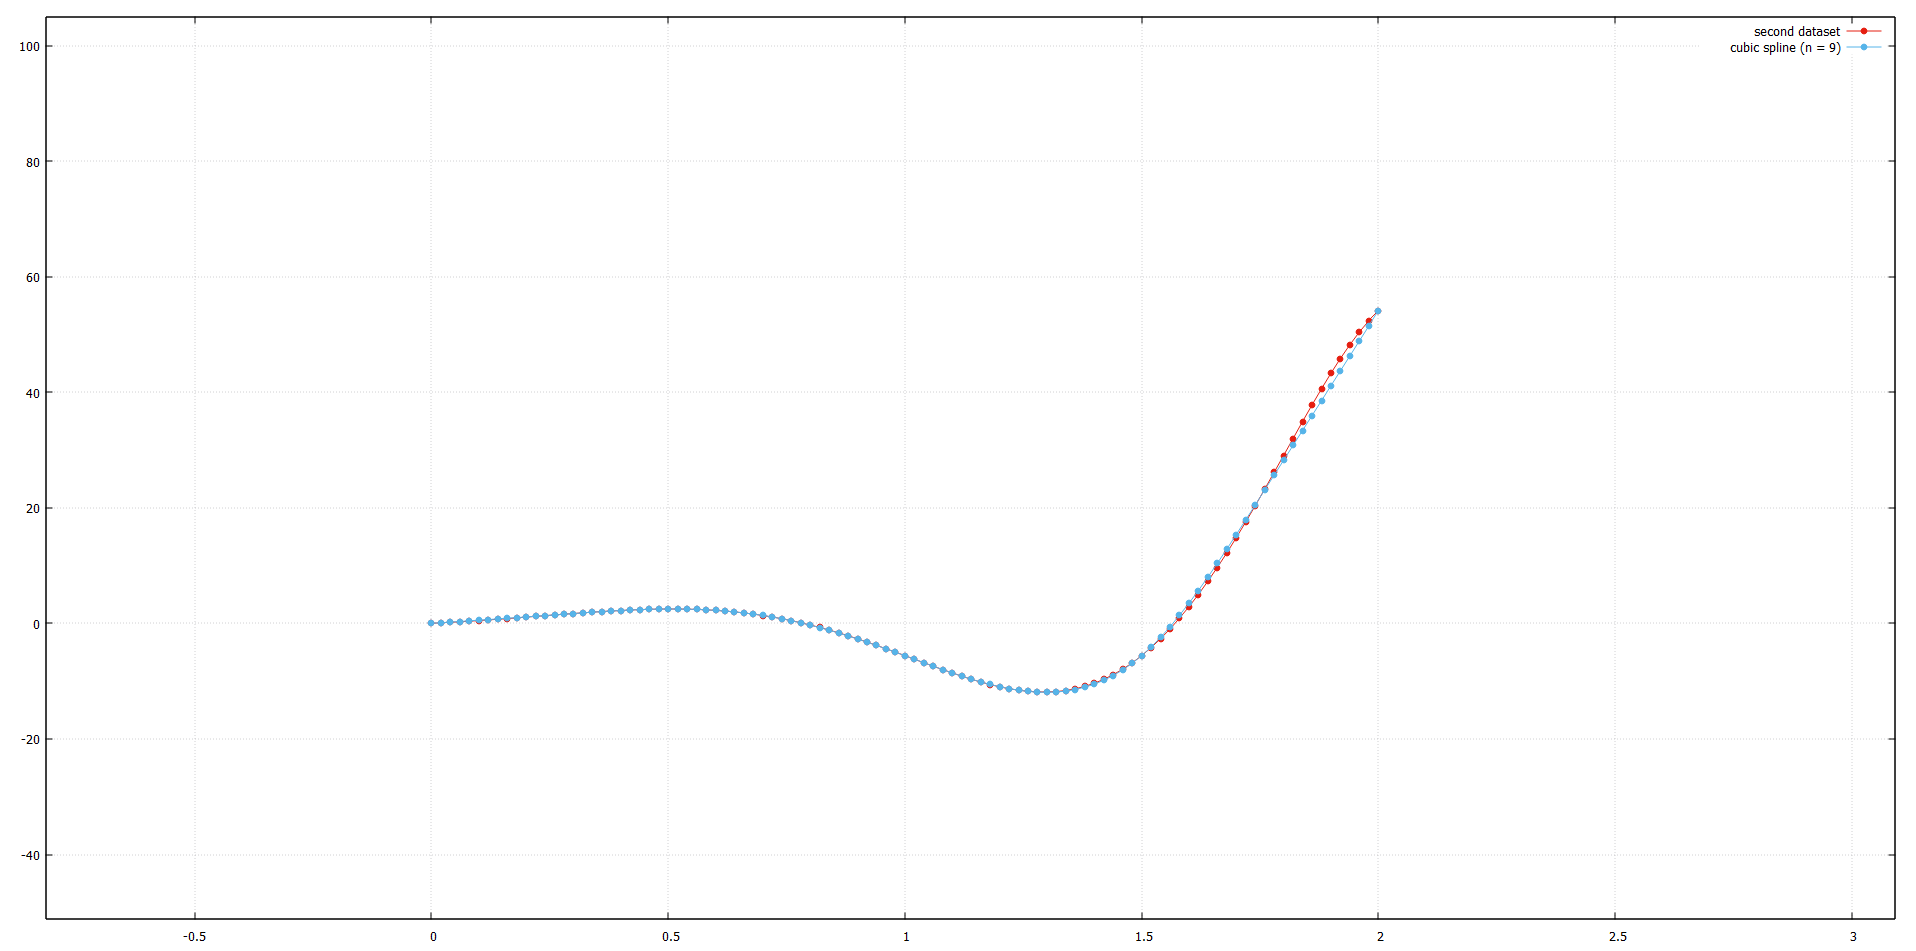
\includegraphics[width=\textwidth]{graph/f2_9.png}
        \caption{Cubic spline (n = 9)}
    \end{minipage}%
\end{figure*}

\begin{figure*}[h]
    \centering
    \begin{minipage}{0.8\textwidth}
        \centering
        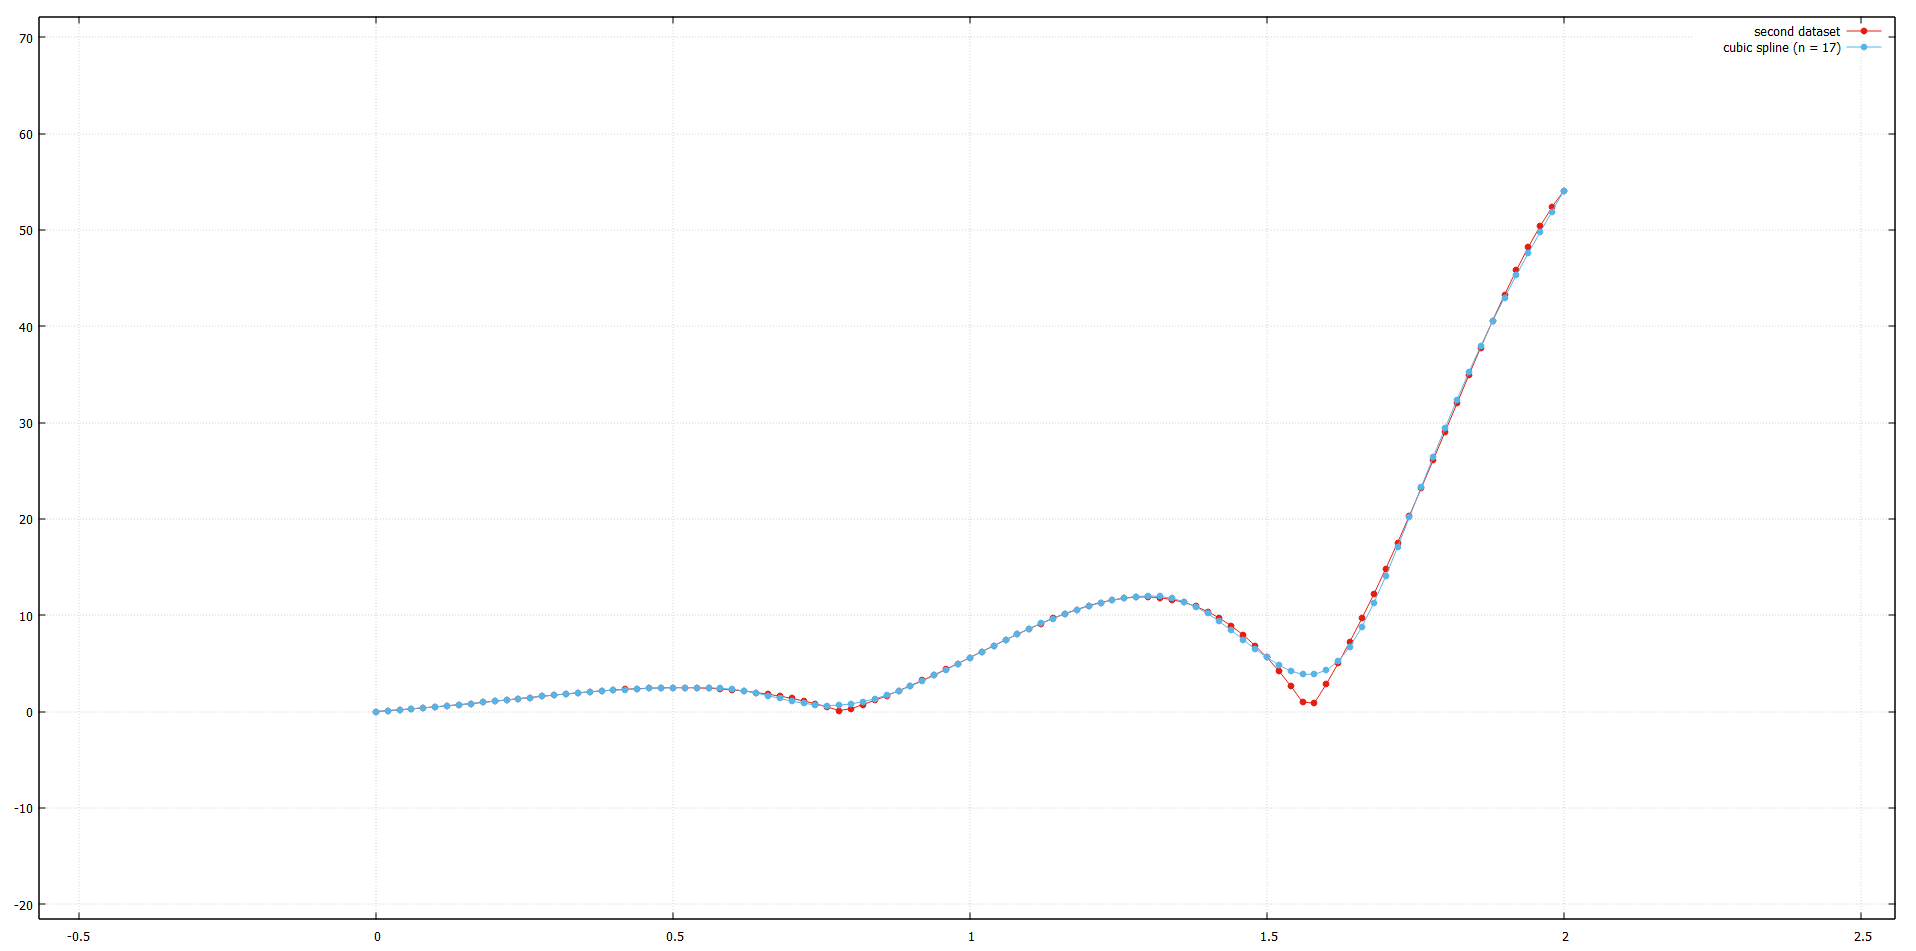
\includegraphics[width=\textwidth]{graph/f2_17.png}
        \caption{Cubic spline (n = 17)}
    \end{minipage}%
\end{figure*}

\begin{figure*}[h]
    \centering
    \begin{minipage}{0.8\textwidth}
        \centering
        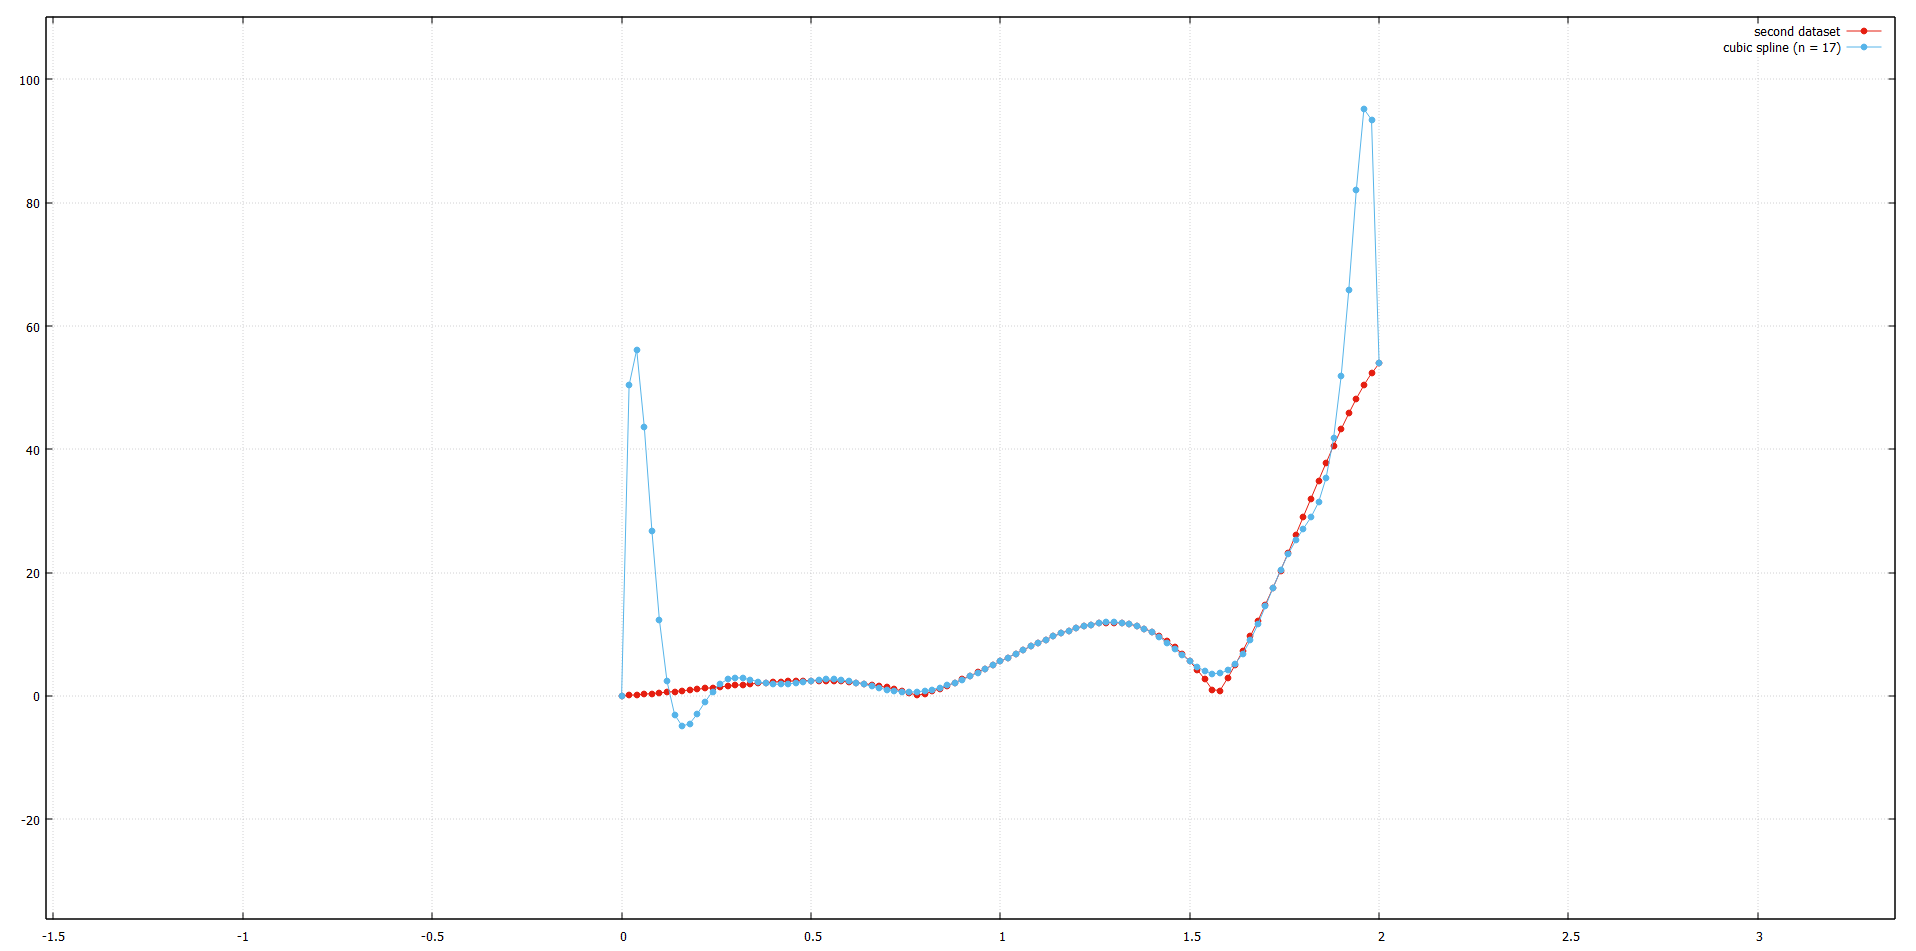
\includegraphics[width=\textwidth]{graph/f2_poly_17.png}
        \caption{Проблемы с интерполированием полиномом Лагранжа на первом наборе данных}
    \end{minipage}%
\end{figure*}

\section*{Итоги}

\begin{enumerate}
    \item \textbf{Функция \(f_1\)}, интерполянт Лагранжа:
    \begin{itemize}
        \item При 3--5 узлах результат более-менее точный, ошибка невелика.
        \item При 17 узлах результат становится еще более точным. Однако, вообще говоря, при разных границах отрезка возникает всё же риск эффекта Рунге на краях; однако если взять узлы «равномерно», может понадобиться сгущение на концах отрезка. На втором наборе данных заметно сильное отклонение.
    \end{itemize}
    \item \textbf{Функция \(f_2\)}, кубический сплайн:
    \begin{itemize}
        \item Имеет более лучшую сходимость из-за того, что полином Лагранжа становится не очень эффективным при больших осцилляциях функции
        \item Ошибка при 17 узлах получается весьма небольшой.
    \end{itemize}
\end{enumerate}

\chapter{Применение численных методов на практике}
Задачи интерполяции часто возникают на практике. Среди них можно выделить:
\begin{itemize}
    \item использование интерполяционных методов для данных о каких-либо экспериментах, чтобы «дополнить» недостающие точки для построения непрерывного набора данных;
    \item применение в компьютерной графике и компьютерном зрении, когда нужно улучшить качество изображения или увеличить разрешение, используя интерполяционные методы. Зная данные об изображении (имеем набор цветов пикселей для определенного разрешения), можно его достроить до более точного, посчитав промежуточные значения для пикселей, которые и будут формировать большее разрешение изображения;
    \item использование в метеорологии, где часто нужно «заполнить пропуски» в пространственно-временных измерениях.
\end{itemize}

\noindent Как итог: интерполяция --- важный инструмент в самых разных областях (численный анализ, обработка сигналов, машинное обучение, компьютерная графика). В частности, кусочно-полиномиальная интерполяция сплайнами, благодаря своей устойчивости к эффекту Рунге, является «золотым стандартом» во многих реальных задачах аппроксимации функций.

\bigskip

\chapter*{Заключение}
\addcontentsline{toc}{chapter}{Заключение}

В рамках отчёта выполнено:
\begin{itemize}
    \item Построение интерполяционного полинома Лагранжа для функций \(f_1, f_2\) при разном числе узлов (3, 5, 9, 17).
    \item Получен результат: интерполяция кубическими сплайнами для \(f_2\), оказалась более применимой для второй функции

\end{itemize}

\vspace{10pt}

\noindent Также была показана \textbf{примерная область применения} каждого из методов, включая их сильные стороны и ограничения.

\begin{thebibliography}{9}
\renewcommand{\bibname}{Литература}
\bibitem{samarskiy}
А.\,А. Самарский. \textit{Введение в теорию разностных схем.} М.: Наука, 1971.

\bibitem{kostomarov}
Д.\,П. Костомаров, А.\,П. Фаворский. \textit{Вводные лекции по численным методам.} — М.: Логос, 2004. — 184 с.

\bibitem{samarskiy_intro}
Самарский А.\,А. \textit{Введение в численные методы}. — М.: Наука, 1989. — 416 с.

\end{thebibliography}

\end{document}

